\documentclass[aspectratio=43,english]{beamer} %If you want to create Polish presentation, replace 'english' with 'polish' and uncomment 3-th line, i.e., '\usepackage{polski}'
\usepackage[utf8]{inputenc}
\usepackage{polski} %Uncomment for Polish language
\usepackage{babel}
\usepackage{listings} %We want to put listings

\mode<beamer>{ 	%in 'beamer' mode
	\hypersetup{pdfpagemode=FullScreen}		%Enable Full screen mode
	\usetheme{JuanLesPins} 		%Show part title in right footer
	%\usetheme[dark]{AGH}                 		%Use dark background
	%\usetheme[dark,parttitle=leftfooter]{AGH}  	%Use dark background and show part title in left footer
}
\mode<handout>{	%in 'handout' mode
	\hypersetup{pdfpagemode=None}		
	\usepackage{pgfpages}
  	\pgfpagesuselayout{4 on 1}[a4paper,border shrink=5mm,landscape]	%show 4 slides on 1 page
  	\usetheme{boxes}
  	\addheadbox{structure}{\quad\insertpart\hfill\insertsection\hfill\insertsubsection\qquad} 	%content of header
 	\addfootbox{structure}{\quad\insertauthor\hfill\insertframenumber\hfill\insertsubtitle\qquad} 	%content of footer
}

\AtBeginPart{ %At begin part: display its name
	\frame{\partpage}
} 


%%%%%%%%%%% Configuration of the listings package %%%%%%%%%%%%%%%%%%%%%%%%%%
% Source: https://en.wikibooks.org/wiki/LaTeX/Source_Code_Listings#Using_the_listings_package
%%%%%%%%%%%%%%%%%%%%%%%%%%%%%%%%%%%%%%%%%%%%%%%%%%%%%%%%%%%%%%%%%%%%%%%%%%%%
\lstset{ %
  backgroundcolor=\color{white},   % choose the background color
  basicstyle=\footnotesize,        % the size of the fonts that are used for the code
  breakatwhitespace=false,         % sets if automatic breaks should only happen at whitespace
  breaklines=true,                 % sets automatic line breaking
  captionpos=b,                    % sets the caption-position to bottom
  commentstyle=\color{green},      % comment style
  deletekeywords={...},            % if you want to delete keywords from the given language
  escapeinside={\%*}{*)},          % if you want to add LaTeX within your code
  extendedchars=true,              % lets you use non-ASCII characters; for 8-bits encodings only, does not work with UTF-8
  frame=single,	                   % adds a frame around the code
  keepspaces=true,                 % keeps spaces in text, useful for keeping indentation of code (possibly needs columns=flexible)
  keywordstyle=\color{blue},       % keyword style
  morekeywords={*,...},            % if you want to add more keywords to the set
  numbers=left,                    % where to put the line-numbers; possible values are (none, left, right)
  numbersep=5pt,                   % how far the line-numbers are from the code
  numberstyle=\tiny\color{gray},   % the style that is used for the line-numbers
  rulecolor=\color{black},         % if not set, the frame-color may be changed on line-breaks within not-black text (e.g. comments (green here))
  showspaces=false,                % show spaces everywhere adding particular underscores; it overrides 'showstringspaces'
  showstringspaces=false,          % underline spaces within strings only
  showtabs=false,                  % show tabs within strings adding particular underscores
  stepnumber=2,                    % the step between two line-numbers. If it's 1, each line will be numbered
  stringstyle=\color{cyan},        % string literal style
  tabsize=2,	                   % sets default tabsize to 2 spaces
  title=\lstname,                  % show the filename of files included with \lstinputlisting; also try caption instead of title
                                   % needed if you want to use UTF-8 Polish chars
  literate={?}{{\k{a}}}1
           {?}{{\k{A}}}1
           {?}{{\k{e}}}1
           {?}{{\k{E}}}1
           {�}{{\'o}}1
           {�}{{\'O}}1
           {?}{{\'s}}1
           {?}{{\'S}}1
           {?}{{\l{}}}1
           {?}{{\L{}}}1
           {?}{{\.z}}1
           {?}{{\.Z}}1
           {?}{{\'z}}1
           {?}{{\'Z}}1
           {?}{{\'c}}1
           {?}{{\'C}}1
           {?}{{\'n}}1
           {?}{{\'N}}1
}
%%%%%%%%%%%%%%%%%


\title{Metody Obliczeniowe w Nauce i Technice}
\author{Marian Bubak, PhD}
\date{}
\institute[AGH]{
	Institute of Computer Science\\ul. Kawiory 21\\30-055 Krakow\\
	Poland\\
	\url{http://www.icsr.agh.edu.pl/~mownit/}
}


\usepackage{amsmath}
\usepackage{mathtools}
\subtitle{3 - Interpolacja}
\begin{document}
	\maketitle
	%%%%%%%%%%%%%%%%
	\begin{frame}{Plan wykładu}
		\tableofcontents
	\end{frame}
	%%%%%%%%%%%%%%%%
	\section{Zadanie interpolacji}
	\begin{frame}{3.1 Zadanie interpolacji}

	\begin{figure}[h]
			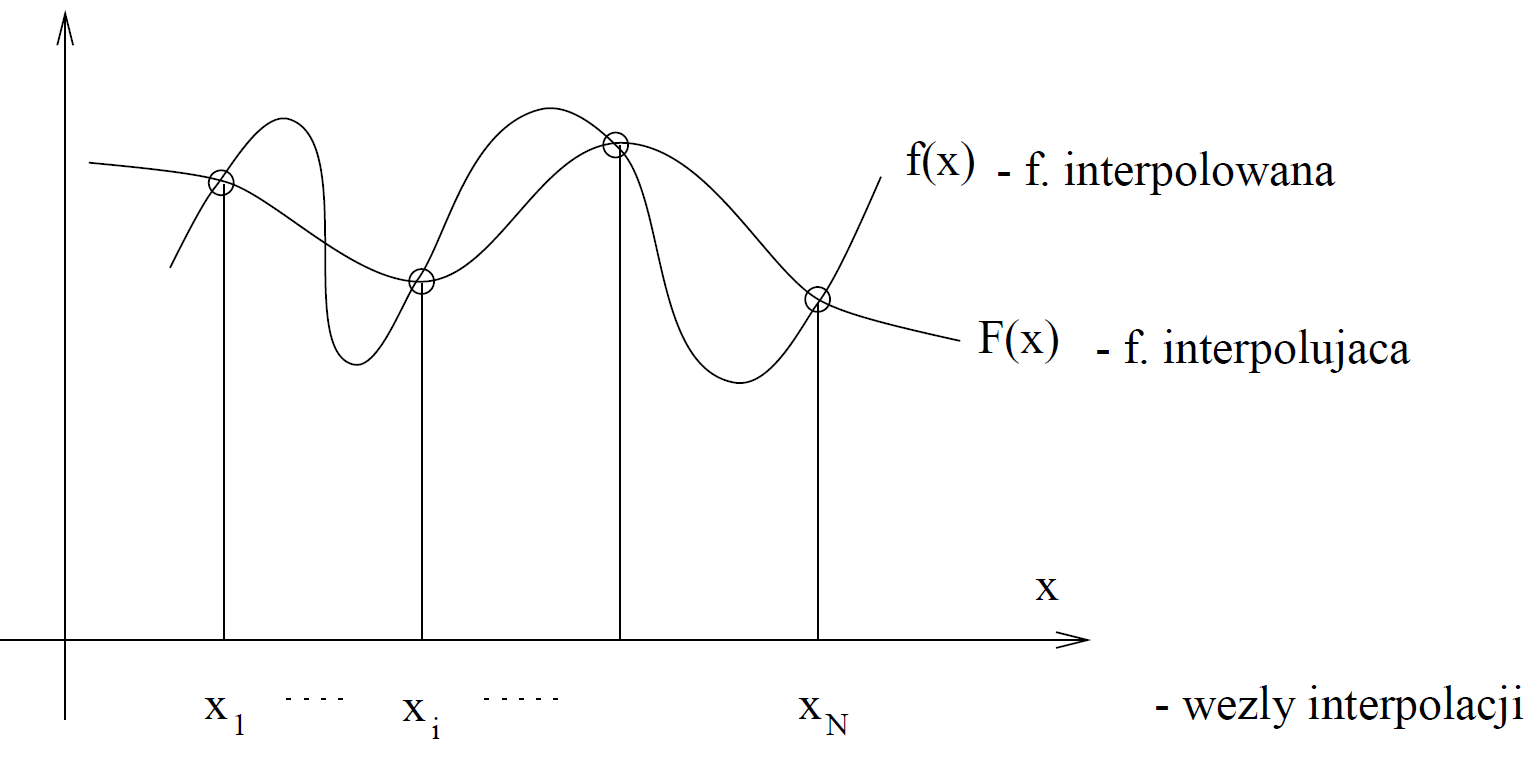
\includegraphics[width=1 \linewidth]{img/3/interpol_3_1}
	\end{figure}
    \end{frame}
    
    \begin{frame}
	\textcolor{blue}{Dane:}

	\begin{itemize}
	\item $[a,\ b]$

	\item $\{(x_{i},\ f_{i}=f(x_{i})),\ i=1,\ 2,\ .\ .\ .\ ,\ N\}$
	$\newline$
    \end{itemize}
	\textcolor{blue}{Szukane:}
	\begin{itemize}
	\item $F(x)$ - funkcja interpolująca $\rightarrow $ wartości w $x \neq x_{i}$ \\
    \item $E(x)$ - oszacowanie błędu interpolacji
    \end{itemize}
    $\newline$
    pod warunkiem: \\
    $F(x_{i}) = f_{i}$ - takie same w węzłach
    $\newline$ \\
    Odmiana:
    poza $f(x_{i})$ dane także $f^{(k)}(x_{i})$
    
	\end{frame}
    %%%%%%%%%%%%%%%%%%%%%%%
    \section{Klasy funkcji interpolujących}
	\begin{frame}{3.2 Klasy funkcji interpolujących}

	

	Funkcje o ,,rozsądnym przebiegu między węzłam'',\ tj.:

	\setlength\parindent{24pt} 
\begin{itemize}
    \item gładkość (smoothness),
    
    \item prostota (simplicity);
\end{itemize}
	\noindent a takimi są np.:
\begin{itemize}
	\item wielomiany algebraiczne,

	\item wielomiany trygonometryczne,

	\item funkcje wymierne,

	\item funkcje sklejane (spline).
\end{itemize}
    \end{frame}


    %%%%%%%%%%%%%%%%%%%%%%%
    \section{Przydatność interpolacji}
	\begin{frame}{3.3 Przydatność interpolacji}
	
\begin{itemize}

	\item zagęszczenie tablic (zamiast długiej tablicy krótka tablica $+$ krótka procedura interpolacyjna), \newline
    \item zastępowanie skomplikowanych funkcji np. wielomianami, \newline
    \item znajdowanie $f^{(k)}(x)$ w punktach pośrednich, \newline
    \item całkowanie numeryczne, \newline
    \item rozwiązywanie równiań różniczkowych, \newline
    \item interpolacjia odwrotna: wyznaczanie $x$, któremu odpowiada $y = f(x)$ nie występujaca w tablicy.
     \end{itemize}

	\end{frame}
    %%%%%%%%%%%%%%%%%%%%%%%
    \section{Wielomiany algebraiczne}
	\begin{frame}{3.4 Wielomiany algebraiczne \\ 3.4.1 Cechy wielomianów algebraicznych}


	\begin{itemize}
	\item łatwość obliczeń $+, *, \displaystyle \frac{d}{dx}, \displaystyle \int dx\ldots $ \newline


    \begin{block}{Twierdzenie Weierstrass'a}
    Dla dowolnej $f(x)$ ciągłej na $[a,\ b]$ (skończonym), i każdego

    $\epsilon>0$ istnieje wielomian $W_{n}(x)$, $n=n(x)$ taki, że:

	\[ \max\limits_{x \in [a,b]}|f(x)-W_{n}(x)|<\epsilon \]


  	\end{block}
    \end{itemize}

	\end{frame}

    \begin{frame}{3.4.2 Postać naturalna wielomianu}
    \begin{block}{}
		$$W(x)=\sum_{i=0}^{n}a_{i}x^{i},\ a_{i}=\frac{W^{(i)}(0)}{i!}$$
    \end{block}
        \begin{itemize}
        \item postać naturalna - rozwinięcie Maclaurina \\

        \item $a_{i}$ - znormalizowane pochodne
		\end{itemize}
    \end{frame}

    \begin{frame}{3.4.3 Algorytm W.G. Hornera}
    \setlength\parindent{24pt}
	\begin{block}{}
		$$W(x)=(\ldots(a_{n}x+a_{n-1})x+\cdots+a_{1})x+a_{0}$$
	\end{block}
	czyli:

	$\qquad W_{n}=a_{n},$ \\

	$\qquad W_{i}=W_{i+1}x+a_{i}, \quad i=n-1, n-2, \cdots , 0$ \\

	$\qquad W(x)=W_{0}$ \\

	otrzymujemy:
	\begin{itemize}
	\item $n-$mnożeń, $n -$dodawań
	\item numerycznie poprawny (wskaźnik kumulacji $\approx 2n+1$)
	\end{itemize}
    \vspace{3mm}
	$\quad$\textbf{Zadanie:} sprawdzić.
    \end{frame}

    \begin{frame}{3.4.4 Postać Newtona}
    \begin{block}{}
	$$W(x)\ =\ \sum_{k=0}^{n}b_{k}p_{k}(x)\ ;$$
	\end{block}
	$$p_{0}(x)\ =\ 1$$

	$$p_{k}(x)\ =\ (x-x_{0})(x-x_{1})\ldots(x-x_{k-1})$$

    \end{frame}

    %%%%%%%%%%%%%%%%%%%%%%%
    \section{Wielomian Interpolacyjny Lagrange'a}

\begin{frame}{3.5 Wielomian Interpolacyjny Lagrange'a \\ 3.5.1 Interpolacja liniowa}


$P_{1}(x)$ -- przez $(x_{0},\ y_{0})$ i $(x_{1},\ y_{1})$
$$
P_{1}(x)=\underbrace{\frac{(x-x_{1})}{(x_{0}-x_{1})}}_{L_0(x)}y_{0}+\underbrace{\frac{(x-x_{0})}{(x_{1}-x_{0})}}_{L_1(x)}y_{1}=\sum_{k/0}^{1}L_{k}(x)f(x_{k})
$$
\begin{itemize}
\item wielomian stopnia $\leq 1$

\item $x=x_{0}\rightarrow P(x_{0})=y_{0}$ \\
$x=x_{1}\rightarrow P(x_{1})=y_{1}$ \\
$L_{k}(x_{l})=\delta_{k,l}$ \\
\end{itemize}
\begin{flushright}Czy jest jedynym takim wielomianem?\end{flushright}

\end{frame}


\begin{frame}{3.5.2 Wielomian $\mathrm{n}$-tego stopnia}


przez $x_{0}, x_{1}, x_{2}$, . . . , $x_{n}$

$L_{k}(x_{l})=\delta_{k,l}=\left\{\begin{array}{l}
0,\ k\neq l\ (\star)\ \\
1,\ k=l\ (\star\star)
\end{array}\right. \text{f. ,,wymierna''} $

$(\star)\rightarrow$ licznik 
$=(x-x_{0})(x-x_{1})\ldots(x-x_{k-1})^{\downarrow}(x-x_{k+1})\ldots(x-x_{n})$

$(\star\star)\rightarrow$ mianownik 
$=(x_{k}-x_{0})(x_{k}-x_{1})\ldots(x_{k}-x_{k-1})(x_{k}-x_{k+1})\ldots(x_{k}-x_{n})$

LIP:

$$L_{k}(x)=\prod_{i/0,i\neq k}^{n}\frac{x-x_{i}}{(x_{k}-xi)}\ , \quad P_{n}(x)=\sum_{k/0}^{n}L_{k}(x)f(x_{k})$$

\textbf{Zadanie:} wykres $L_{k}(x)$ , sprawdzić $\displaystyle \sum_{k/0}^{n}L_{k}(x)=1$
\end{frame}


\begin{frame}{3.5.3 Jednoznaczność rozwiązania}

$P_{n}(x)$ -wiel. stopnia $\leq n$, przechodzący przez punkty:
$$
\{(x_{i},\ f_{i}),\ i=0,\ 1,\ 2,\cdots ,\ n\ ,\ x_{i}\neq x_{j}\}
$$

\begin{block}{Twierdzenie}

Jest tylko jeden taki wielomian.\\
\vspace{2mm}
\textbf{Dane:} Niech $\exists q_{n}(x)\neq P_{n}(x)$ , przez w/w punkty,

$\Rightarrow r_{n}(x)=P_{n}(x) \quad -q_{n}(x)$ -wiel. stopnia $\leq n$
$$
 \: -r_{n}(x_{i})=0,\ i=\underbrace{0,1, \dots, n}_{n+1}
$$
$$
\Rightarrow r_{n}(x)\equiv 0
$$
\end{block}
\end{frame}

\begin{frame}{3.5.4 Błąd interpolacji Lagrange'a}

\begin{block}
{Dygresja: Twierdzenie uogólnione $Tw$. {\it Rollea}:}

Założenia:
\begin{center}
1. $f\in C[a,\ b],$ \\
2. $f\in C^{n}(a,\ b),$  \\
3. $f=0\: w\: (n+1)\: $różnych$ \:punktach$
\end{center}


Teza:
$$
\exists c\in(a,\ b):f^{(n)}(c)=0
$$
\end{block}
\textbf{Dowód:}

Twierdzenie Rolle'a kolejno do:

$f \rightarrow f'\mathrm{o}$ {\it n}- zerach

$f' \rightarrow f'' \:o\:(n-1)$ --zerach \newline
$f^{(n-1)} \rightarrow f^{(n)} o\: 1$ \: --zerze
 \end{frame}
 
 \begin{frame}
 \begin{figure}[h]
			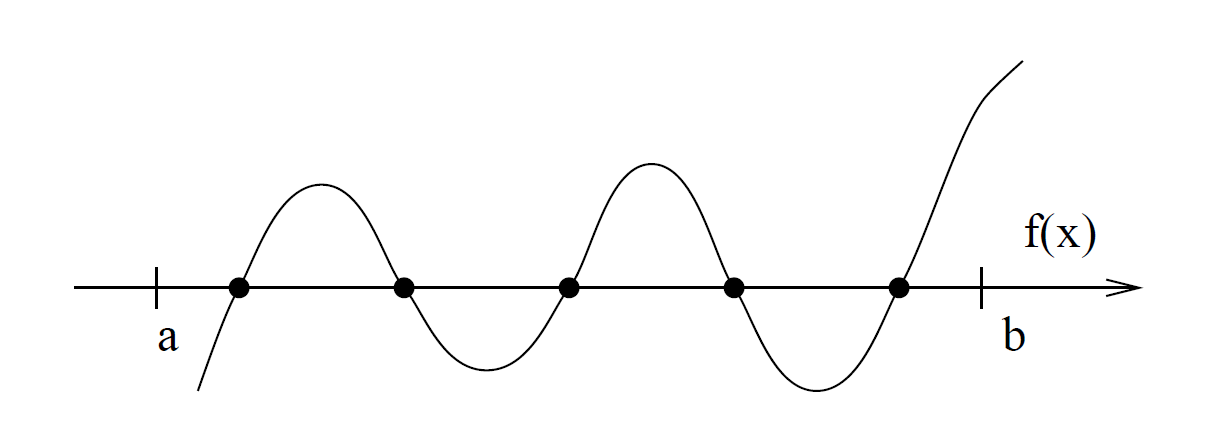
\includegraphics[width=1 \linewidth]{img/3/interpol_3_5}
	\end{figure}
Rysunek 3.2: Funkcja spelniająca zalożenia uogólnionego tw. Rolle'a 
 \end{frame}
 
 
 
 \begin{frame}

Założenia:

\begin{itemize}
\item $x_{0}, x_{1}$, . . . , $x_{n}\in[a,\ b]$ różne punkty 
\item $P_{n}(x)$ -wiel. interpolacyjny Lagrange'a 
\item $f\in C^{(n+1)}[a,\ b]$
\end{itemize}

\begin{block}
{Teza:}
$$\forall x\in[a,\ b]\ \exists\eta(x)\in(a,\ b)\ :$$

$$f(x)=P_{n}(x)+\frac{f^{n+1}(\eta(x))}{(n+1)!}\prod_{i/0}^{n}(x-x_{i})\ (\star)$$
\end{block}

\end{frame}

\begin{frame}
Dane:

$x=x_{k}, k=0$, 2, . . . , $n \rightarrow f(x_{k})=P_{n}(x_{k})\Rightarrow$dowolny $\eta$ spelnia $(\star)$ \newline
- dla ustalonego $x\neq x_{k}, k=0$, 1, . . . , $n\Rightarrow g(t)$ , $[a,\ b]$ :

$$g(t)=f(t)-P_{n}(t)-[f(x)-P_{n}(x)]\prod_{i/0}^{n}\frac{t-x_{i}}{x-x_{i}}$$

$$
 \left. \begin{array}{ll}
f\in C^{(n+1)}[a,\ b] \\
P\in C^{\infty}[a,\ b]\\
x\neq x_{k}
\end{array} \right \} \Rightarrow g(t)\in C^{(n+1)}[a,\ b] 
$$

$\fbox{$t=x_{k}:$}$

$$g(x_{k})=\underbrace{f(x_{k})-P_{n}(x_{k})}_{=0}-[f(x)-P_{n}(x)]\underbrace{\prod_{i/0}^{n}\frac{x_{k}-x_{i}}{x-x_{i}}}_{=0}=0$$

\end{frame}

\begin{frame}
$\fbox{$t=x:$}$
$$
g(x)=f(x)-P_{n}(x)-[f(x)-P_{n}(x)]\underbrace{\prod_{i/0}^{n}\frac{x-x_{i}}{x-x_{i}}}_{=1}=0
$$
$\Rightarrow g(t)$ ma $(n+2)$ miejsc zerowych: $x, x_{0}, x_{1}$, . . . , $x_{n}$ \newline \newline
Zastosowanie twierdzenia Rolle'a:


$$\begin{array}{ll}
0=g^{(n+1)}(\displaystyle \eta)= \\
f^{(n+1)}(\eta)-\underbrace{P_{n}^{(n+1)}(\eta)}_{=0}-[f(x)-P_{n}(x)]\frac{d^{n+1}}{dx^{n+1}} \left \{\prod_{i/0}^{n}\frac{t-x_{i}}{x-x_{i}} \right \}_{t=\eta}  \end{array}$$


 \end{frame}
 
 \begin{frame}
 

$\displaystyle \prod_{i/0}^{n}\frac{t-x_{i}}{x-x_{i}}=\frac{t^{n+1}}{\prod_{i/0}^{n}(x-x_{i})}+at^{n}+\cdots$
$$
f^{(n+1)}(\eta)=[f(x)-P_{n}(x)]\frac{(n+1)!}{\prod_{i/0}^{n}(x-x_{i})}
$$
\textbf{błąd interpolacji Lagrange'a:}
$$
f(x)=P_{n}(x)+\underbrace{\frac{f^{n+1}(\eta(x))}{(n+1)!}\prod_{i/0}^{n}(x-x_{i})}_{- por.\: reszta\: Taylora!}
$$


\textbf{Zadanie:} Wyprowadź r. Taylora powyższą metodą \\
\end{frame}

\begin{frame}
\begin{itemize}
\item Alternatywny zapis LIP: $(x_{0},\ x_{1},\ \ldots,\ x_{n})$ :
\end{itemize}
$\displaystyle \omega(x)=\prod_{k/0}^{n}(x-x_{k})$

$P_{n}(x)=\displaystyle \omega(x)\sum_{k/0}^{n}\frac{f(x_{k})}{(x-x_{k})\omega ^{'}(x_{k})}$ \\
\vspace{5mm}

\textbf{Zadanie:} Sprawdzić
 
 \end{frame}

    %%%%%%%%%%%%%%%%%%%%%%%
    \section{Algorytm Neville'a}
\begin{frame}
{3.6 Algorytm Neville'a}

O algorytmie Neville'a: Data Analysis BriefBook5 (autor: Rudolf K. Bock,CERN)
{\it http://www.cern.ch/RD11/rkb/AN16pp/node182.html} \newline

\textcolor{blue}{Istota:} budowa tablicy wielomianów coraz wyższych stopni.
\begin{figure}[h]
			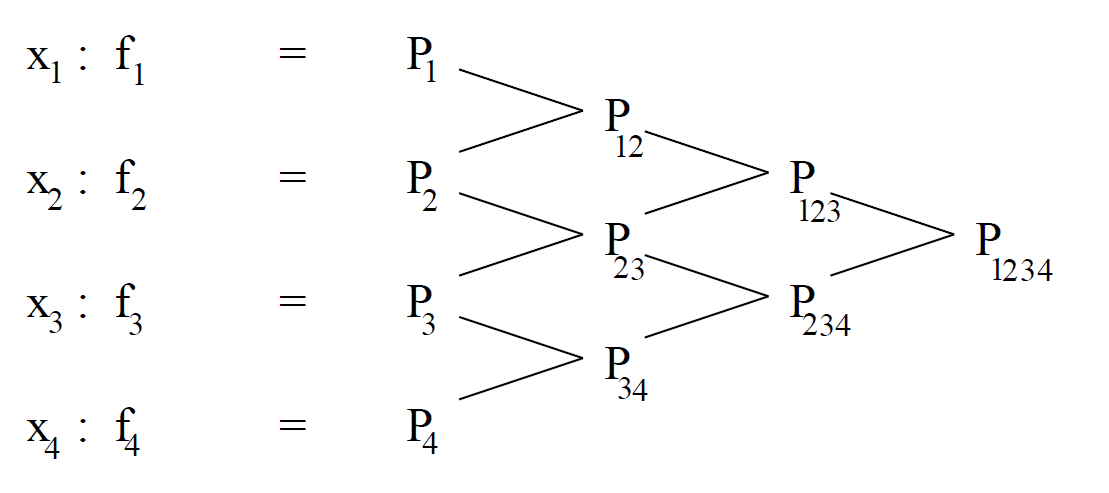
\includegraphics[scale = 0.28]{img/3/interpol_3_6}
	\end{figure}
Rysunek 3.3: Ilustracja metody Neville'a
\end{frame}

\begin{frame}
$P_{1}, P_{2}, P_{3}, P_{4}$ -- wiel. stopnia $0$, przechodzący przez $(x_{i},\ f_{i})$ ,

$P_{12}, P_{23}, P_{34}$ -- wartość w $x$ dla wielomianów stopnia 1, przechodzącego przez pary punktów, \\
\vspace{4mm}
\textbf{Rekurencyjne zapełnianie tabeli:}

$P_{i(i+1)\ldots(i+m)}=\displaystyle \frac{1}{x_{i}-x_{i+m}}(x-x_{i+m})P_{i(i+1)\ldots(i+m-1)}+(x_{i}-x)P_{(i+1)(i+2)\ldots(i+m)}$

\begin{itemize}
\item otrzymamy wielomian stopnia $N-1$

\item zgodny z $f(x)$ w węzłach, np.:
$$
P_{12}=\frac{(x-x_{2})P_{1}-(x-x_{1})P_{2}}{x_{1}-x_{2}}\ ;\ P_{12}(x_{1})=P_{1};P_{12}(x_{2})=P_{2}
$$

\end{itemize}

\end{frame}

\begin{frame}


Wygodniej-- różnice między pokoleniami:
$$
C_{m,i}=P_{i\cdots(i+m)}-P_{i\cdots(i+m-1)}\ ;\ D_{m,i}=P_{i\cdots(i+m)}-P_{i\cdots(i+m)}
$$
$$
D_{m+1,i}\ =\ \frac{x_{i+m+1}-x}{x_{i}-x_{i+m+1}}(C_{m,i+1}-D_{m,i})
$$
$$
C_{m+1,i}\ =\ \frac{x_{i}-x}{x_{i}-x_{i+m+1}}(C_{m,i+1}-D_{m,i})
$$
\vspace{3mm}

Końcowy wynik -- suma różnic wzdłuż wybranej ścieżki. \\
Dodatkowo otrzymujemy oszacowanie błędu. \\
\vspace{3mm}
\textbf{Zadanie}: sprawdzić poprawność, napisać algorytm, \\
oszacować błąd.
\end{frame}

    %%%%%%%%%%%%%%%%%%%%%%%
    \section{3.7 Metoda ilorazów różnicowych (divided differences)}
\begin{frame}
{3.7 Metoda ilorazów różnicowych (divided differences)}

Interesuje nas nie wartość, a postać wielomianu.

$P_{n}(x)-\text{LIP, stp. } \leq n$, zgodny z $f(x)$ w $\{x_{0},\ x_{1},\ .\ .\ .\ ,\ x_{n}\}$

Można go zapisać w postaci:
\begin{equation*}\begin{split}
P_{n}(x)=a_{0}+a_{1}(x-x_{0})+a_{2}(x-x_{0})(x-x_{1})+ \\
\cdots+a_{n}(x-x_{0})(x-x_{1})\cdots(x-x_{n-1})
\end{split}
\end{equation*}

$a_{0}$: $a_{0}=P_{n}(x_{0})=f(x_{0})$

$a_{1}$ : $f(x_{0})+a_{1}(x_{1}-x_{0})=P_{n}(x_{1})=f(x_{1}) \Rightarrow$

$$
a_{1}=\frac{f(x_{1})-f(x_{0})}{x_{1}-x_{0}}
$$
\end{frame}

\begin{frame}
Wprowadzamy notację:
\begin{itemize}
\item 0-wy iloraz różnicowy wzgl. $x_{i}$ : $f[x_{i}]=f(x_{i})$ \\
pozostałe - indukcyjnie:

\item 1-szy:
$$
f[x_{i},\ x_{i+1}]=\frac{f[x_{i+1}]-f[x_{i}]}{x_{i+1}-x_{i}}
$$
Gdy zaś określone są ilorazy aż do $(k-1)$ , czyli
$$
f[x_{i},\ x_{i+1},\ x_{i+k-1}] \: i \: f[x_{i+1},\ x_{i+2},\ x_{i+k}]
$$
\item to wtedy k-ty iloraz różnicowy:
\end{itemize}
$$
f[x_{i},\ x_{i+1}, ...\ x_{i+k}]=\frac{f[x_{i+1},x_{i+2},\ldots.x_{i+k}]-f[x_{i},x_{i+1},\ldots.x_{i+k-1}]}{x_{i+k}-x_{i}}
$$
\end{frame}

\begin{frame}
Interpolacyjny wzór Newtona z ilorazami różnicowymi:
$$
P_{n}(x)=f[x_{0}]+\sum_{k/1}^{n}f[x_{0},\ x_{1},\ .\ .\ .\ ,\ x_{k}](x-x_{0})\cdots(x-x_{k-1})
$$
\textbf{Zadanie}: Policzyć $a_{2}, a_{3}$, zapisać algorytm.

\end{frame}

\begin{frame}

\begin{block}
{Twierdzenie iloraz różnicowy a pochodna}

Założenia:
\begin{itemize}
\item $f\in C^{n}[a,\ b]$
\item $x_{0}, x_{1}$, . . . , $x_{n}\in[a,\ b] $ i są różne
\end{itemize}

Teza:
$$
\exists\eta\in(a,\ b)\ f[x_{0},\ x_{1},\ .\ .\ .\ ,\ x_{n}]=\frac{f^{(n)}(\eta)}{n!}
$$
\end{block}
\vspace{5mm}

\textbf{Zadanie:} Podać dowód.
\end{frame}

\begin{frame}
\textbf{Węzły równoodległe}

$h=x_{i+1}-x_{i} \quad i=0, 1, ..., n-1$ \\
$x=x_{0}+s*h$ \\
$x-x_{i}=(s-i)h$ \\

\begin{gather*} P_{n}(x)=P_{n}(x_{0}+s*h) =\\
   f[x_{0}]+s*h*f[x_{0}, x_{1}]+s(s - 1)h^{2}f[x_{0},x_{1},x_{2}]+ \\
+ \cdots +s(s-1)\cdots(s-n+1)h^{n}f[x_{0},x_{1},\dots ,x_{n}]
\end{gather*}

\begin{gather*}
\binom{s}{k}=\displaystyle \frac{s(s-1)\ldots(s-k+1)}{k!}\\
P_{n}(x)=P_{n}(x_{0}+sh)=\sum_{k=0}^{n}(_{k}^{s})k!h^{k}f[x_{0}, x_{1}, \cdots ,x_{k}]
\end{gather*}
\end{frame}

\begin{frame}
\begin{itemize}
\item Newton forward divided-difference formule {\it (r. progresywna)} \\
\vspace{2mm}
$f[x_{0},\displaystyle \ x_{1},\cdots,\ x_{k}]=\frac{1}{k!h^{k}}\triangle^{k}f(x_{0})$ \\
\vspace{3mm}
$\rightarrow$ różnica progresywna rzędu $k$
\end{itemize}

$$P_{n}(x)=\displaystyle \sum_{k=0}^{n}(_{k}^{s})\triangle^{k}f(x_{0})$$
\end{frame}

    %%%%%%%%%%%%%%%%%%%%%%%
    \section{Interpolacja Hermite'a}
\begin{frame}
{3.8 Interpolacja Hermite'a}

Więcej o metodzie i jej autorze \\
(autor: Shayne Waldrom,University of Auckland):\\
\vspace{5mm}
https://www.math.auckland.ac.nz/$\sim$waldron/Hermite/hermite.html
\end{frame}

\begin{frame}
{3.8.1 Przypadek szczególny}

$\{(x_{i}, f_{i}, f_{i}^{'}); i=1,2, \dots, N; x_{i}\neq x_{j}, i\neq j\}$
$$
P_{2N-1}(x)=\sum_{i/1}^{N}\alpha_{i}(x)f(i)+\sum_{i/1}^{N}\beta_{i}(x)f_{i}'
$$
$$
\alpha_{i}\ =\ [1-2(x-x_{i})\Phi_{i}'(x_{i})]\Phi_{i}^{2}(x)
$$
$$
\beta_{i}\ =\ (x-x_{i})\Phi_{i}^{2}(x)
$$
\begin{center}
$\Phi_{i}(x) = \displaystyle \prod_{j/1,j\neq i}^{N}\frac{x-x_{j}}{x_{i}-x_{j}}, i=1, 2,\dots, N$
$$
\Phi_{i}'(x_{i})\ =\ [\Phi_{i}'(x)]_{x_{i}}
$$
\end{center}
\textbf{Zadanie:} sprawdzić.


\end{frame}

\begin{frame}
$$
\alpha_{i}(x_{j})\ =\ [1-2(x_{j}-x_{i})\Phi_{i}'(x_{i})]\delta_{ij}^{2}=\delta_{ij}
$$
$$
\beta_{i}(x_{j})\ =\ (x_{j}-x_{i})\delta_{ij}^{2}=0
$$
$\Rightarrow$ wielomian przechodzi przez $(x_{j},\ f_{j})$ , $j=1,2, \dots, N$ \\
\vspace{3mm}
$\alpha_{i}^{l}(x_{j})\ =\ [1-2(x_{j}-x_{i})\Phi_{i}(x_{i})]2\delta_{ij}\Phi_{i}'(x_{j})-2\Phi_{i}^{l}(x_{i})\delta_{ij}=0$ \\
\vspace{3mm}
$\beta_{i}'(x_{j})\ =\ (x_{j}-x_{i})2\delta_{ij}\Phi_{i}'(x_{j})+\delta_{ij}=\delta_{ij}$

$$
\Rightarrow\ P_{2N-1}'(x_{j})=f_{j}'
$$
\begin{flushright}$\rightarrow$ wzór zmodyfikowany \end{flushright}
\end{frame}

\begin{frame}
{3.8.2 Ogólnie}

\textcolor{blue}{Dane:}
\begin{itemize}
\item $k+1$ różnych węzłów: $x_{0}, x_{1}, \dots, x_{k}$

\item liczby naturalne $m_{0}, m_{1},\dots , m_{k}, \displaystyle \sum_{i/1}^{k}m_{i}=n+1$
\end{itemize}
\textcolor{blue}{Szukamy:}

dla dowolnej funkcji $ f(\rightarrow$liczb {\it $f_{i}^{(j)}$}$)$ wielomianu $H_{n}$ stopnia $\leq n,$ \\
takiego, że:

$H_{n}^{(j)}(x_{i})=f^{(j)}(x_{i})$ \quad dla $i=0, 1, \dots , k$
\begin{center}
$j=0, 1, \dots, m_{i-1}$
\end{center}
( $m_{i}=1\rightarrow$ interpolacja Lagrange'a)
\end{frame}

\begin{frame}
\textcolor{blue}{Rozwiązanie:} \\
\vspace{2mm}
$s(i)=\left\{\begin{array}{l}
0,\ i=0\\
m_{0}+m_{1}+\cdots+m_{i-1},\ i>0
\end{array}\right.$
\vspace{2mm}

$0\leq l\leq n:l=s(i)+j$

$p_{s(0)}(x)=1$

$p_{s(i)+j}(x)=(x-x_{0})^{m_{0}}(x-x_{1})^{m_{1}}\ldots(x-x_{i-1})^{mi-1}(x-x_{i})^{j}(\star)$ \\
gdzie: $i=0, 1, \dots, k; \: j=1, 2, \dots , m_{i-1}$ \\
\vspace{3mm}
Szukany wielomian interpolacyjny:
$$
H_{n}(x)=\sum_{l/0}^{n}b_{l}p_{l}(x)=\sum_{i/0}^{k}\sum_{j/0}^{m_i-1}b_{s(i)+j}p_{s(i)+j}(x)
$$
\end{frame}

\begin{frame}
współczynniki $b_{l}$:


$l$ - ustalone, $l=s(i)+j$
$$
H_{n}(x)=\underbrace{A(x)}_{b_{0},{b_{1},\ldots,b}_{l-1}}+b_{l}p_{l}(x)+\underbrace{B(..x)}_{b_{l+1},\ldots,b_{n}}(\star\star)
$$
ale: $(\mathrm{z}\star)$
$$
l=s(i)+jp_{l}(x)=p_{s(i)}(x)(x-x_{j})^{j}
$$
$
$różniczkując$(\star\star)
$
$$
H_{n}^{(j)}(x_{i})=A^{(j)}(x_{i})+b_{l}p_{s(i)}(x_{i})j!
$$
korzystając $\mathrm{z}$:
$$
H_{n}^{(j)}(x_{i})=f^{(j)}(x_{i})
$$
mamy:
$$
b_{l}=\frac{f^{(j)}(x_{i})-A^{(j)}(x_{i})}{p_{s(i)}(x_{i})_{j}j!}
$$

\end{frame}
    %%%%%%%%%%%%%%%%%%%%%%%
    \section{3.9 Efekt Rungego}
\begin{frame}
{3.9 Efekt Rungego}

(C. Runge, 1901)
$$
y(x)=\frac{1}{1+25x^{2}},\ x\in[-1,\ 1]
$$
Występuje, gdy:
\begin{itemize}
\item interpolujemy wielomianami

\item węzły interpolacyjne są równoodległe
\end{itemize}

Rada praktyczna:

\begin{itemize}
\item zaczynać od interpolacji liniowej,

\item zwiększać liczbę węzłów i stopień wielomianu, aż do ustabilizowania istotnych miejsc.
\end{itemize}


Sposób -- \textbf{interpolacja przedziałowa}.
\begin{itemize}
\item Katastrofalna rozbiezność dla $0.726\leq|x|<1$.

\item Lecz bardzo dobra zbieżność w strefie centralnej.
\end{itemize}

(konsekwencja tego, że zadanie to jest {\itźle uwarunkowane})
\end{frame}
\begin{frame}
\begin{figure}[h]
			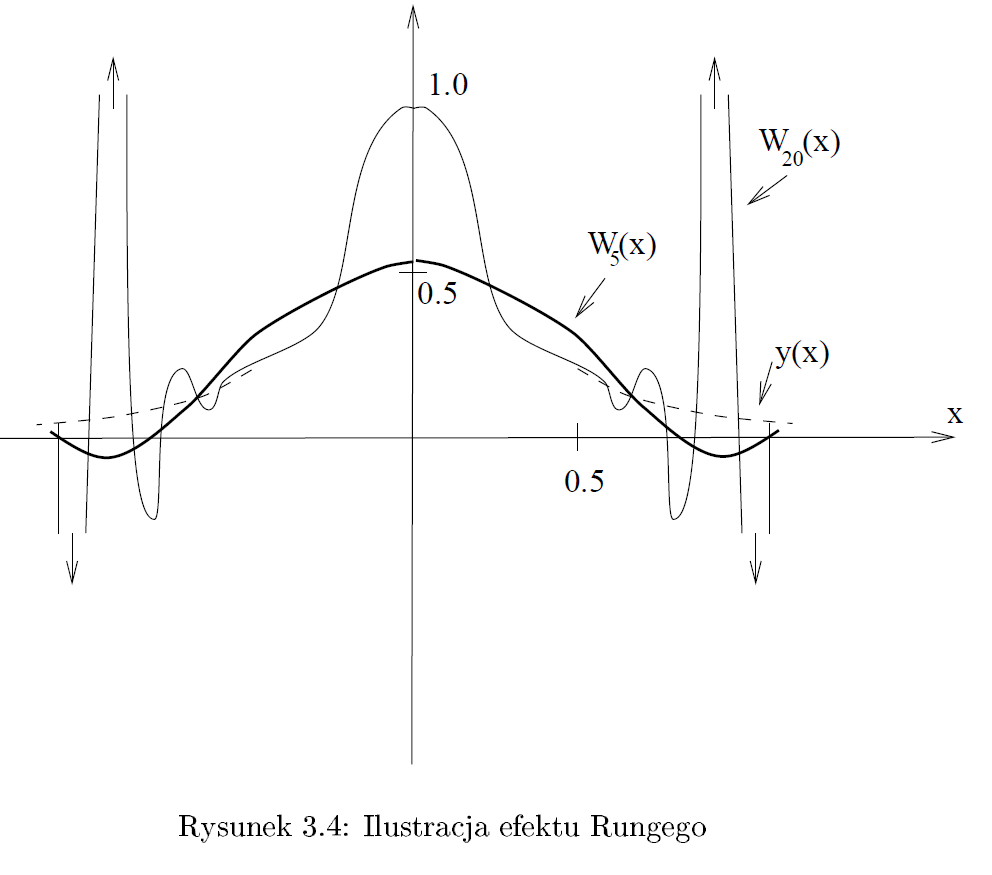
\includegraphics[scale=0.35]{img/3/interpol_3_9}
	\end{figure}
\end{frame}



\begin{frame}{Bibliografia}
      \begin{thebibliography}{9}
              \setbeamertemplate{bibliography item}[book]
              \bibitem[RUDOLF]{Rudolf}{Rudolf, K. Bock \newblock O wielomianach w Data Analysis BriefBook \newblock CERN}
              \setbeamertemplate{bibliography item}[book]
              \bibitem[RUDOLF]{Rudolf}{Rudolf, K. Bock \newblock O regule Hornera w Data Analysis BriefBook \newblock CERN}
              \setbeamertemplate{bibliography item}[book]
              \bibitem[RUDOLF]{Rudolf}{Rudolf, K. Bock \newblock O algorytmie Neville'a w Data Analysis BriefBook \newblock CERN}
      \end{thebibliography}
  \end{frame}
  
\end{document}

 